\section{Results}
\label{sec:results}
In \Cref{sec:ablations} we first focus on understanding the impact of
the main components of our training setup on performance as measured
by recall@10 and triplet accuracy. Afterwards in
\Cref{sec:minimal-pairs} we switch our attention to the targetted
evaluation via minial pairs.
\todo{GC: We really should have at least 3 runs of each configuration with a different random seed.}


\subsection{Ablations}
\label{sec:ablations}
For completeness, we report results on both the dialog and narration
data. However, it should be kept in mind that in the case of the
narration data the scores are not confounded by speaker-based clues
and thus the scores on narration are those that indicate to what extent to
model learns aspects of utterance meaning.

\todo{GC: Generate and insert results on test data}
\subsubsection{Pre-training and Fine-tuning}
Results on different pre-training configurations are shown in
\Cref{fig:pretraining}.
\begin{figure}[htb]
	\centering
	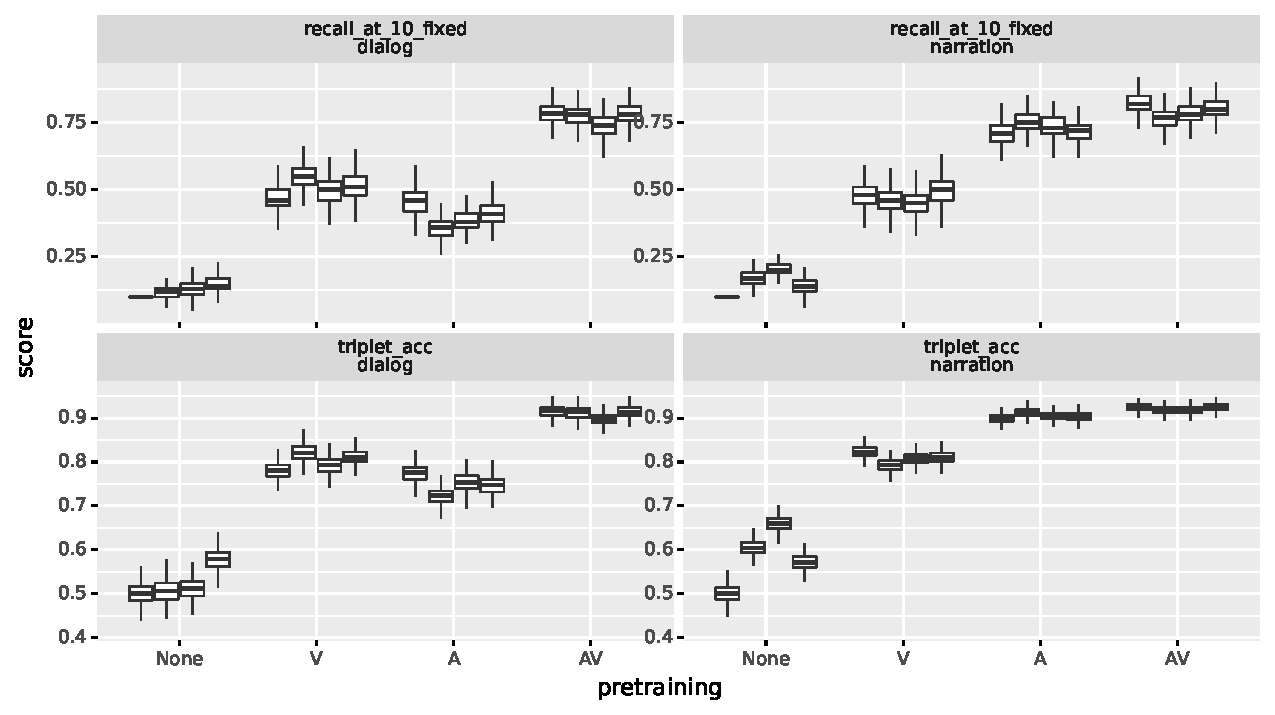
\includegraphics[width=\columnwidth]{results/ablations/pretraining.pdf}
	\caption{Effect of pre-training on performance on the dialog
          and narration validation data. The top row shows recall@10;
          the bottom row triplet accuracy.}
	\label{fig:pretraining}
      \end{figure}

The best overall performance on both the dialog and the narration data is 
achieved with a model where both the video and audio encoder are pre-trained 
before being fine-tuned on our data. The model with no pre-training in
either modality failed to converge and thus performs at random.


On narration data, for both metrics, we see a clear ranking of
configurations from best to worst: (AV) audio and video pre-training,
(A) audio pre-training, (V) video pre-training and (None) no
trainining. Meanwhile for dialog data, the performance between A and V
is comparable.

%A model that is trained on scratch using only our data performs still 
%substantially above chance on all metrics ($0.1$ for recall@10 and $0.5$ for 
%triplet accuracy). \todo{MN: Do we maybe want to add the chance (random 
%guessing) baselines into the plots? }

To further understand and disentangle the effects of audio pre-training and 
fine-tuning, we train a model with frozen parameters of the 
\textsc{wav2vec} module. The effect of this condition is show in \Cref{fig:freeze_wav2vec}.
\begin{figure}[htb]
  \centering
  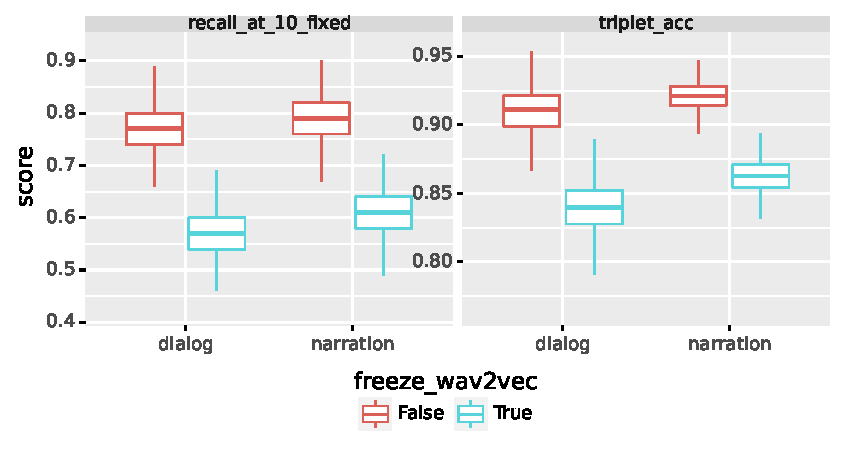
\includegraphics[width=\columnwidth]{results/ablations/freeze_wav2vec.pdf}
  \caption{Effect of freezing the parameters of the \textsc{wav2vec}
    module on model performance, on the dialog and narration
    validation data. The top row shows recall@10; the bottom row
    triplet accuracy.}
  \label{fig:freeze_wav2vec}
\end{figure}
We find without fine-tuning of the \textsc{wav2vec} module, performance decreases substantially 
on both metrics. In other words, best performance is only achieved with pre-trained and 
fine-tuned models.


\subsubsection{Jitter}
Next, we evaluate a model that has been trained with varying video and audio 
lengths (\textsc{jitter}). For fair comparison, we report recall@10 for both 
\textsc{fixed} and \textsc{jitter} validation configurations.
As seen in \Cref{fig:jitter}, the effect of \textsc{jitter} is only
minor and that performance is comparable. \todo{GC: Insert reference
  to results with jitter for minimal pair scenario.}
\begin{figure}[htb]
	\centering
	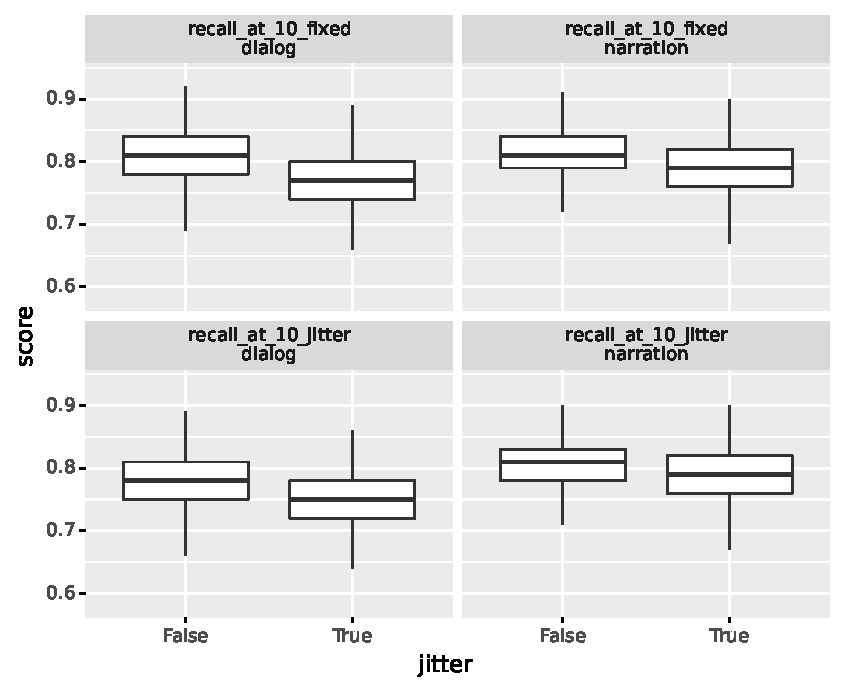
\includegraphics[width=\columnwidth]{results/ablations/jitter.pdf}
	\caption{Effect of jitter on model performance, on the dialog
          and narration validation data. The top row shows recall@10;
          the bottom row triplet accuracy.}
	\label{fig:jitter}
\end{figure}



\subsubsection{Temporal Information}
Finally, we explore the role of the temporal nature of the visual
modality.  \Cref{fig:static} compares the model with the regular video
encoder with one using the \textsc{static} baseline encoder. Across
all metrics, we observe substantial performance drops for the
\textsc{static} model, which has access to the same video frames, but
does not have access to their temporal ordering. \todo{GC: Note that a
  confounding factor here is that the static encoder is pre-trained on
  ImageNet rather than Kinetics. Maybe we should instead compare
  models without video pre-training.}

\begin{figure}[htb]
  \centering
  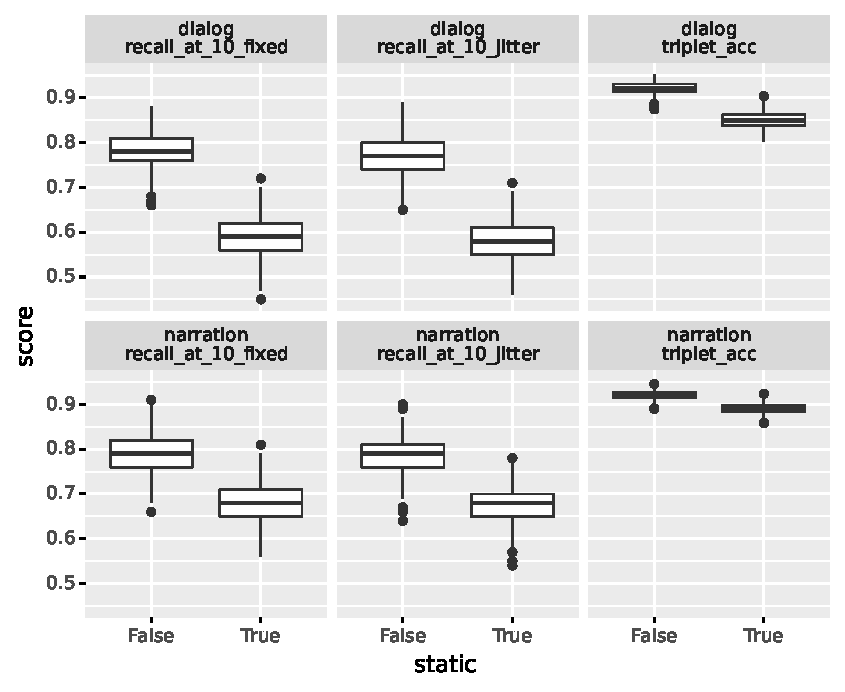
\includegraphics[width=\columnwidth]{results/ablations/static.pdf}
  \caption{Effect of temporal information on model performance, on the dialog
          and narration validation data. The top row shows recall@10;
          the bottom row triplet accuracy.}
  \label{fig:static}
\end{figure}


\subsection{Minimal Pairs}
\label{sec:minimal-pairs}
As a first baseline, we evaluate a model which is pre-trained but not
fine-tuned on our dataset. The resulting performance is, as expected,
close to chance level: 0.538.\todo{MN: add baselines: model that is
  completely untrained, and model where only the attention pooling
  layers are finetuned}

Additionally, we evaluate a model using static (image)
data instead of video. The average accuracy is 0.705 . Finally, the
best performing model according to the performance metrics (ID 68,
audio and video pretraining) achieves an average targeted triplets
accuracy of 0.745.

\Cref{fig:accuracy_targeted_triplets_nouns} and
\ref{fig:accuracy_targeted_triplets_verbs} show per-word
accuracy for nouns and verbs, respectively.
We perform boostrapping (n\_resampling = 100) to estimate mean and standard deviation for each accuracy score.

We further compute correlations between the per-word accuracy and two 
possible predictors of age of acquisition: frequency and concreteness. 
We do not find any significant correlation between the model's per-word 
accuracy and word concreteness or input frequency of a word in the 
training data.\todo{MN: verify correlations for final versions. GC:
  maybe skip them unless they are strong.}



\todo{GC: Can we get rid of the text on top of these per-word plots.}
\begin{figure*}[htb]
  \centering
  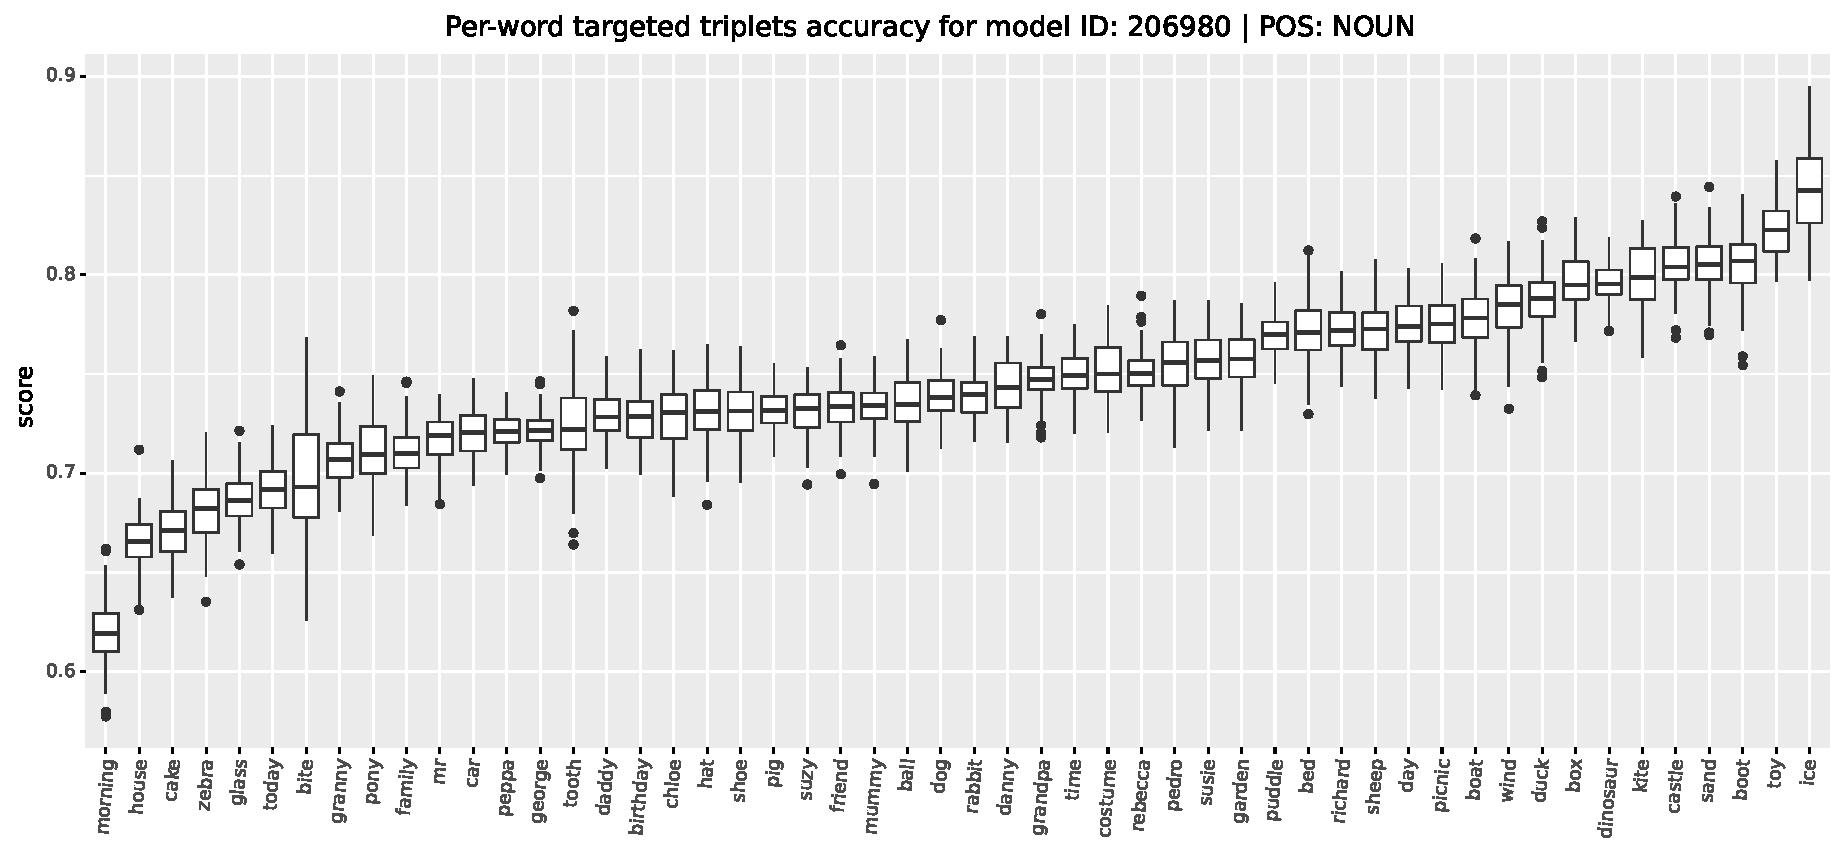
\includegraphics[width=\textwidth]{results/targeted_triplets/results_per_word_version_206980_NOUN.pdf}
  \caption{Per-word accuracies on the minimal pairs evaluation data for nouns.}
  \label{fig:accuracy_targeted_triplets_nouns}
\end{figure*}

\begin{figure*}[htb]
  \centering
  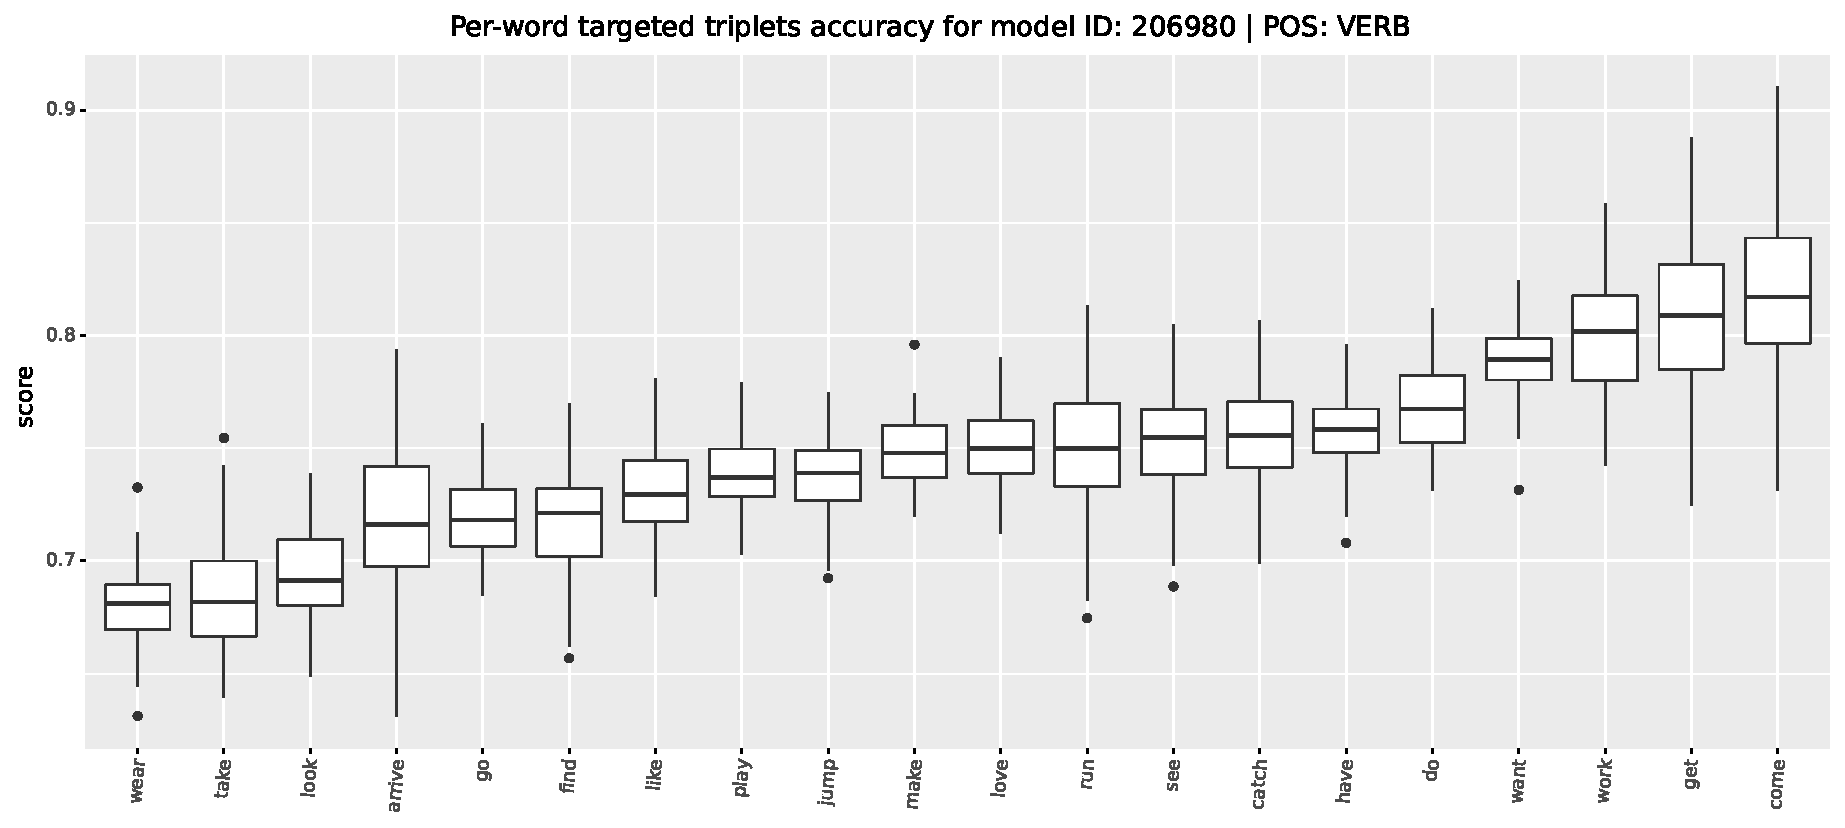
\includegraphics[width=\textwidth]{results/targeted_triplets/results_per_word_version_206980_VERB.pdf}
  \caption{Per-word accuracies on the minimal pairs evaluation data
    for verbs.}
  \label{fig:accuracy_targeted_triplets_verbs}
\end{figure*}
